\documentclass[conference]{IEEEtran}
\usepackage{times}

% numbers option provides compact numerical references in the text.
\usepackage[numbers]{natbib}
\usepackage{multicol}
\usepackage[bookmarks=true]{hyperref}

\usepackage{graphicx} % more modern
%\usepackage{epsfig} % less modern
\usepackage{subfigure}

% For algorithms
\usepackage{algorithm}
\usepackage{algorithmic}
\usepackage{amsmath}
\usepackage{amssymb}
% Include other packages here, before hyperref.
\usepackage{color}
\usepackage{setspace}
\usepackage{wrapfig}
\usepackage{dsfont}

\usepackage[it,small]{caption}


\newcommand{\argmax}{\operatorname{arg\,max}}
\newcommand{\argmin}{\operatorname{arg\,min}}
\newcommand{\todo}[1]{\textcolor{blue}{\textbf{#1}}}
\newtheorem{mydef}{Definition}



\graphicspath{{./images/}}
\usepackage{multirow}
% Some illegal space-saving macros
% \parskip=1pt
  \abovedisplayskip 3.0pt plus2pt minus2pt%
 \belowdisplayskip \abovedisplayskip
\renewcommand{\baselinestretch}{0.97}

\newenvironment{packed_enum}{
\begin{enumerate}
  \setlength{\itemsep}{0pt}
  \setlength{\parskip}{0pt}
  \setlength{\parsep}{0pt}
}
{\end{enumerate}}

\newenvironment{packed_item}{
\begin{itemize}
  \setlength{\itemsep}{0pt}
  \setlength{\parskip}{0pt}
  \setlength{\parsep}{0pt}
}{\end{itemize}}

\newlength\savedwidth
\newcommand\whline[1]{\noalign{\global\savedwidth\arrayrulewidth
                               \global\arrayrulewidth #1} %
                      \hline
                      \noalign{\global\arrayrulewidth\savedwidth}}

% \renewcommand\multirowsetup{\centering}

\newlength{\sectionReduceTop}
\newlength{\sectionReduceBot}
\newlength{\subsectionReduceTop}
\newlength{\subsectionReduceBot}
\newlength{\abstractReduceTop}
\newlength{\abstractReduceBot}
\newlength{\captionReduceTop}
\newlength{\captionReduceBot}
%\newlength{\nameReduceTop}
\newlength{\subsubsectionReduceTop}
\newlength{\subsubsectionReduceBot}
\newlength{\headerReduceTop}
% Negative space for figures set at the bottom of a block of figs
\newlength{\figureReduceBot}

\newlength{\horSkip}
\newlength{\verSkip}

\newlength{\equationReduceTop}

\newlength{\figureHeight}
\setlength{\figureHeight}{1.7in}

%\newlength{\figureFraction}
\setlength{\horSkip}{-.09in}
\setlength{\verSkip}{-.1in}
%\setlength{\figureFraction}{.195}

% figureReduceBot is for figures which are set above text, since latex
% likes putting a lot of space under those
\setlength{\figureReduceBot}{-0.15in}
\setlength{\headerReduceTop}{0in}
%
%\setlength{\subsectionReduceTop}{-0.08in}
%\setlength{\subsectionReduceBot}{-0.05in}
\setlength{\subsectionReduceTop}{-0.02in}
\setlength{\subsectionReduceBot}{-0.02in}
%\setlength{\sectionReduceTop}{-0.03in}
%\setlength{\sectionReduceBot}{-0.03in}
\setlength{\sectionReduceTop}{-0.02in}
\setlength{\sectionReduceBot}{-0.01in}
\setlength{\subsubsectionReduceTop}{-0.06in}
\setlength{\subsubsectionReduceBot}{-0.05in}
%
%
%\setlength{\figureHeight}{1.5in}
\setlength{\abstractReduceTop}{-0.05in}
\setlength{\abstractReduceBot}{-0.10in}
%
%

\setlength{\equationReduceTop}{-0.1in}

%\setlength{\nameReduceTop}{-0.05in}


\setlength{\captionReduceTop}{-0.06in}
\setlength{\captionReduceBot}{-0.07in}



\pdfinfo{
   /Author (Homer Simpson)
   /Title  (Robots: Our new overlords)
   /CreationDate (D:20101201120000)
   /Subject (Robots)
   /Keywords (Robots;Overlords)
}

\begin{document}

% paper title
\title{Supplementary Material For \\ rCRF: Recursive Belief Estimation over CRFs in RGB-D Activity Videos}

% You will get a Paper-ID when submitting a pdf file to the conference system
%\author{Author Names Omitted for Anonymous Review. Paper-ID 63}
\author{
\authorblockN{Ozan Sener}
\authorblockA{School of Electrical \& Computer Eng. \\ Cornell University}
\and
\authorblockN{Ashutosh Saxena}
\authorblockA{Department of Computer Science \\ Cornell University}
}


\maketitle

\IEEEpeerreviewmaketitle

\section{Introduction}
In this supplementary material, we give the detailed derivation of the posterior belief we state in equation (8) of the main paper as well as the detailed algorithm to solve the optimization problem in equation (10) of the main paper. We also present the experimental results we did not include in the main paper due to the space limit. Furthermore, we explain the details of the computational-efficiency experiment we conducted in order to obtain the results in Table~3 of the main paper.

\section{Supplementary Results}
\subsection{Computational-Efficiency of the Inference}
We evaluated the computational-efficiency of our algorithm experimentally by recording its run-time. While recording the run-time, we did not include the feature extraction and pre-processing times since feature extraction and pre-processing steps are identical for all the competing algorithms. In other words, the recorded numbers are the inference time of the algorithms. We perform our experiments on an Intel i7 3.0 GHz laptop with 6Gb RAM running Ubuntu operating system using Python programming language. While implementing the algorithms, we only used a single core. Therefore, optimizing and parallelizing the code will give future gains.

\noindent\textbf{Inference time during detection:}
We recorded the runtime of the inference algorithm for each temporal segment while estimating the belief for observed frames in the detection setting. We present the results in Table~\ref{speed1}.

Since the optimization algorithm, we define in (main paper 8) uses the inference procedure repeatedly for each sample, we expect to have a constant \emph{number of diverse samples} multiplicative factor in our computation time. As shown in Table~\ref{speed1}, resulting inference time is approximately ten times the MAP solution although the belief is over $M=15$ diverse samples. We believe this is due to the effective initialization of the mixed integer program with the previous results while iteratively computing the samples. Moreover, temporal segments are longer than 1 second long hence the resulting algorithm is still real-time.
\begin{table}[h!]
  \centering
  \vspace{-2mm}
\caption{Computation time for computing a belief over $M=15$ samples per temporal segment excluding pre-processing.}
\vspace{-2mm}
\resizebox{\columnwidth}{!}{
  \begin{tabular}{|cc|cc|}
    \hline
  MAP Sol. \cite{hemaIJRR} \;  & \; $30ms$    \; \; & \; \;  Full Belief \;  & \;   $367ms$ \\ \hline
\end{tabular}}
  \vspace{-1mm}
  \label{speed1}
\end{table}

\noindent\textbf{Inference time during anticipation:}
We experiment over the 3 seconds into the future anticipation setting and summarize the results in the Table~\ref{speed}. We observed that our method had average computation time of $1.41s$ and \cite{hemaAnt} had average computation time of $34.1s$. This behavior is the result of efficient and accurate sampling of the belief space. Since our samples are more accurate, we need fewer samples than ATCRF \cite{hemaAnt}. Hence, our computation time is significantly better. Indeed, our inference algorithm for anticipation is operating at about 2X real-time.
\begin{table}[h!]
  \centering
  \vspace{-2mm}
\caption{Computation time for anticipating 3 seconds in the future excluding pre-processing.}
\vspace{-2mm}
\resizebox{\columnwidth}{!}{
  \begin{tabular}{|cc|cc|}
    \hline
  ATCRF \cite{hemaAnt} \; \; & \; \; 34.1s  \; \;  \; & \; \; \;  rCRF \; \; & \; \;  1.41s \\ \hline
\end{tabular}}
  \vspace{-1mm}
  \label{speed}
\end{table}

%\subsection{More on the Effect of Anticipation Horizon}
%In addition to the analysis over the effect of anticipation horizon on the accuracy of the object affordance, here we also present the effect of the anticipation horizon on the accuracy of the activity. We computed the average micro-precision of our method and competing ones for anticipation horizons between 1 and 10 seconds and plotted in Figure~\ref{antHor}. General trend of the accuracy curve in the Figure~\ref{antHor} is similar to the object affordance one in the main paper. Therefore, the accuracy over the activity also suggests that recursive modeling is necessary for the belief estimation. On the other hand, one major difference is that all algorithms have similar accuracy values over activities whereas the accuracy over the object affordances varies significantly among the algorithms. We believe this is due to the dimensionality of the space. Activity space has dimension $10^{T}$ whereas the object affordance space has dimension $12^{T\cdot M}$ where $T$ is the length of the video and $M$ is the number of objects. Since the dimension of the object affordance space is significantly larger, recursive modeling and diversity is more crucial.
\subsection{More Visual Results}
We also include additional visual results for activity anticipation in Figure~\ref{abcd} covering various environments. Similar to the visual results in the main paper, we anticipate four temporal segments into the future. Each segment is between 1 to 3 seconds long and the activity at the middle of the segment is anticipated via rCRF using the rest of the video. We present the belief of each anticipated segment as well as the middle frame of the segment. Please note that the visual frames are not visible to the algorithm and only included for evaluation purposes.
\begin{figure}[ht]
\footnotesize
%\begin{singlespace}
\begin{tabular}{p{3mm}@{}l}
\begin{tabular}{l}
\rotatebox[origin=r]{90}{\;\;\;\;\;\;Middle Frame}\\
\rotatebox[origin=l]{90}{Belief\;\;}
\end{tabular}
&
\begin{tabular}{p{3.2cm}p{3.2cm}p{3.2cm}p{3.2cm}}
\includegraphics[width=0.24\textwidth]{seg0} &
\includegraphics[width=0.24\textwidth]{seg1} &
\includegraphics[width=0.24\textwidth]{seg2} &
\includegraphics[width=0.24\textwidth]{seg3}  \\ %\\%\begin{tabular}{p{3.6cm}p{3.6cm}p{3.6cm}p{3.6cm}}
\includegraphics[width=0.24\textwidth, height=8mm]{s0} &
\includegraphics[width=0.24\textwidth, height=8mm]{s1} &
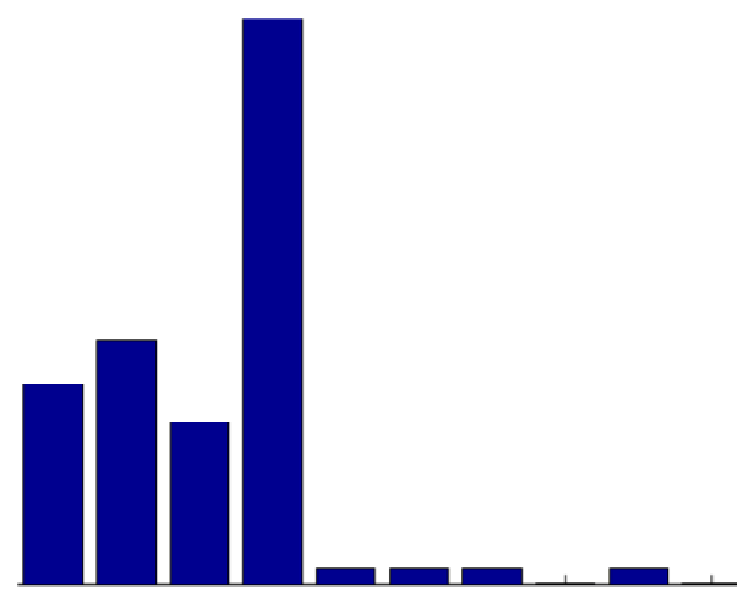
\includegraphics[width=0.24\textwidth, height=8mm]{s2} &
\includegraphics[width=0.24\textwidth, height=8mm]{s3}  \\
\vspace{-10mm}\hspace{0mm}\scalebox{0.72}{
\rotatebox[origin=r]{90}{reaching}\hspace{0.9mm}
\rotatebox[origin=r]{90}{moving}\hspace{0.9mm}
\rotatebox[origin=r]{90}{pouring}\hspace{0.9mm}
\rotatebox[origin=r]{90}{eating}\hspace{0.9mm}
\rotatebox[origin=r]{90}{drinking}\hspace{0.9mm}
\rotatebox[origin=r]{90}{opening}\hspace{0.9mm}
\rotatebox[origin=r]{90}{placing}\hspace{0.9mm}
\rotatebox[origin=r]{90}{closing}\hspace{0.9mm}
\rotatebox[origin=r]{90}{null}\hspace{0.9mm}
\rotatebox[origin=r]{90}{cleaning}}&
\vspace{-10mm}\hspace{-0.9mm}\scalebox{0.72}{
\rotatebox[origin=r]{90}{reaching}\hspace{0.9mm}
\rotatebox[origin=r]{90}{moving}\hspace{0.9mm}
\rotatebox[origin=r]{90}{pouring}\hspace{0.9mm}
\rotatebox[origin=r]{90}{eating}\hspace{0.9mm}
\rotatebox[origin=r]{90}{drinking}\hspace{0.9mm}
\rotatebox[origin=r]{90}{opening}\hspace{0.9mm}
\rotatebox[origin=r]{90}{placing}\hspace{0.9mm}
\rotatebox[origin=r]{90}{closing}\hspace{0.9mm}
\rotatebox[origin=r]{90}{null}\hspace{0.9mm}
\rotatebox[origin=r]{90}{cleaning}}&
\vspace{-10mm}\hspace{-0.9mm}\scalebox{0.72}{
\rotatebox[origin=r]{90}{reaching}\hspace{0.9mm}
\rotatebox[origin=r]{90}{moving}\hspace{0.9mm}
\rotatebox[origin=r]{90}{pouring}\hspace{0.9mm}
\rotatebox[origin=r]{90}{eating}\hspace{0.9mm}
\rotatebox[origin=r]{90}{drinking}\hspace{0.9mm}
\rotatebox[origin=r]{90}{opening}\hspace{0.9mm}
\rotatebox[origin=r]{90}{placing}\hspace{0.9mm}
\rotatebox[origin=r]{90}{closing}\hspace{0.9mm}
\rotatebox[origin=r]{90}{null}\hspace{0.9mm}
\rotatebox[origin=r]{90}{cleaning}}&
\vspace{-10mm}\hspace{-0.9mm}\scalebox{0.72}{
\rotatebox[origin=r]{90}{reaching}\hspace{0.9mm}
\rotatebox[origin=r]{90}{moving}\hspace{0.9mm}
\rotatebox[origin=r]{90}{pouring}\hspace{0.9mm}
\rotatebox[origin=r]{90}{eating}\hspace{0.9mm}
\rotatebox[origin=r]{90}{drinking}\hspace{0.9mm}
\rotatebox[origin=r]{90}{opening}\hspace{0.9mm}
\rotatebox[origin=r]{90}{placing}\hspace{0.9mm}
\rotatebox[origin=r]{90}{closing}\hspace{0.9mm}
\rotatebox[origin=r]{90}{null}\hspace{0.9mm}
\rotatebox[origin=r]{90}{cleaning}}
\end{tabular}
\end{tabular}

\vspace{7mm}


\begin{tabular}{p{3mm}@{}l}
\begin{tabular}{l}
\rotatebox[origin=r]{90}{\;\;\;\;\;\;Middle Frame}\\
\rotatebox[origin=l]{90}{Belief\;\;}
\end{tabular}
&
\begin{tabular}{p{3.2cm}p{3.2cm}p{3.2cm}p{3.2cm}}
\includegraphics[width=0.24\textwidth]{eat1} &
\includegraphics[width=0.24\textwidth]{eat2} &
\includegraphics[width=0.24\textwidth]{eat3} &
\includegraphics[width=0.24\textwidth]{eat4}  \\ %\\%\begin{tabular}{p{3.6cm}p{3.6cm}p{3.6cm}p{3.6cm}}
\includegraphics[width=0.24\textwidth, height=8mm]{et1} &
\includegraphics[width=0.24\textwidth, height=8mm]{et2} &
\includegraphics[width=0.24\textwidth, height=8mm]{et3} &
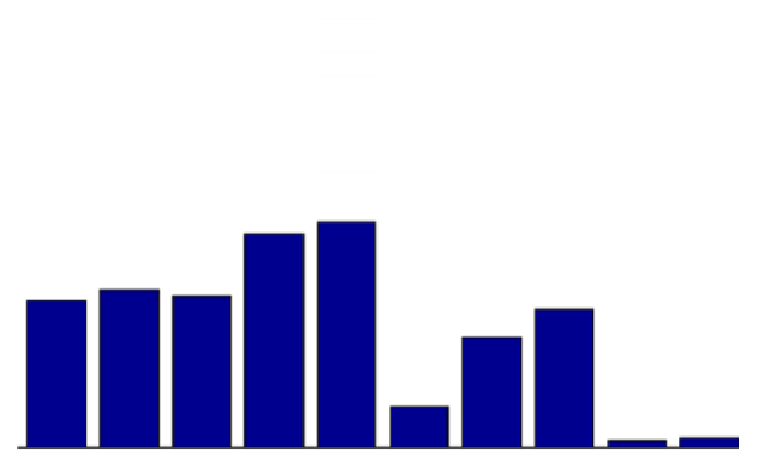
\includegraphics[width=0.24\textwidth, height=8mm]{et4}  \\
\vspace{-10mm}\hspace{0mm}\scalebox{0.72}{
\rotatebox[origin=r]{90}{reaching}\hspace{0.9mm}
\rotatebox[origin=r]{90}{moving}\hspace{0.9mm}
\rotatebox[origin=r]{90}{pouring}\hspace{0.9mm}
\rotatebox[origin=r]{90}{eating}\hspace{0.9mm}
\rotatebox[origin=r]{90}{drinking}\hspace{0.9mm}
\rotatebox[origin=r]{90}{opening}\hspace{0.9mm}
\rotatebox[origin=r]{90}{placing}\hspace{0.9mm}
\rotatebox[origin=r]{90}{closing}\hspace{0.9mm}
\rotatebox[origin=r]{90}{null}\hspace{0.9mm}
\rotatebox[origin=r]{90}{cleaning}}&
\vspace{-10mm}\hspace{-0.9mm}\scalebox{0.72}{
\rotatebox[origin=r]{90}{reaching}\hspace{0.9mm}
\rotatebox[origin=r]{90}{moving}\hspace{0.9mm}
\rotatebox[origin=r]{90}{pouring}\hspace{0.9mm}
\rotatebox[origin=r]{90}{eating}\hspace{0.9mm}
\rotatebox[origin=r]{90}{drinking}\hspace{0.9mm}
\rotatebox[origin=r]{90}{opening}\hspace{0.9mm}
\rotatebox[origin=r]{90}{placing}\hspace{0.9mm}
\rotatebox[origin=r]{90}{closing}\hspace{0.9mm}
\rotatebox[origin=r]{90}{null}\hspace{0.9mm}
\rotatebox[origin=r]{90}{cleaning}}&
\vspace{-10mm}\hspace{-0.9mm}\scalebox{0.72}{
\rotatebox[origin=r]{90}{reaching}\hspace{0.9mm}
\rotatebox[origin=r]{90}{moving}\hspace{0.9mm}
\rotatebox[origin=r]{90}{pouring}\hspace{0.9mm}
\rotatebox[origin=r]{90}{eating}\hspace{0.9mm}
\rotatebox[origin=r]{90}{drinking}\hspace{0.9mm}
\rotatebox[origin=r]{90}{opening}\hspace{0.9mm}
\rotatebox[origin=r]{90}{placing}\hspace{0.9mm}
\rotatebox[origin=r]{90}{closing}\hspace{0.9mm}
\rotatebox[origin=r]{90}{null}\hspace{0.9mm}
\rotatebox[origin=r]{90}{cleaning}}&
\vspace{-10mm}\hspace{-0.9mm}\scalebox{0.72}{
\rotatebox[origin=r]{90}{reaching}\hspace{0.9mm}
\rotatebox[origin=r]{90}{moving}\hspace{0.9mm}
\rotatebox[origin=r]{90}{pouring}\hspace{0.9mm}
\rotatebox[origin=r]{90}{eating}\hspace{0.9mm}
\rotatebox[origin=r]{90}{drinking}\hspace{0.9mm}
\rotatebox[origin=r]{90}{opening}\hspace{0.9mm}
\rotatebox[origin=r]{90}{placing}\hspace{0.9mm}
\rotatebox[origin=r]{90}{closing}\hspace{0.9mm}
\rotatebox[origin=r]{90}{null}\hspace{0.9mm}
\rotatebox[origin=r]{90}{cleaning}}
\end{tabular}
\end{tabular}

\vspace{7mm}

\begin{tabular}{p{3mm}@{}l}
\begin{tabular}{l}
\rotatebox[origin=r]{90}{\;\;\;\;\;\;Middle Frame}\\
\rotatebox[origin=l]{90}{Belief\;\;}
\end{tabular}
&
\begin{tabular}{p{3.2cm}p{3.2cm}p{3.2cm}p{3.2cm}}
\includegraphics[width=0.24\textwidth]{ff2} &
\includegraphics[width=0.24\textwidth]{ff3} &
\includegraphics[width=0.24\textwidth]{ff4} &
\includegraphics[width=0.24\textwidth]{ff5}  \\ %\\%\begin{tabular}{p{3.6cm}p{3.6cm}p{3.6cm}p{3.6cm}}
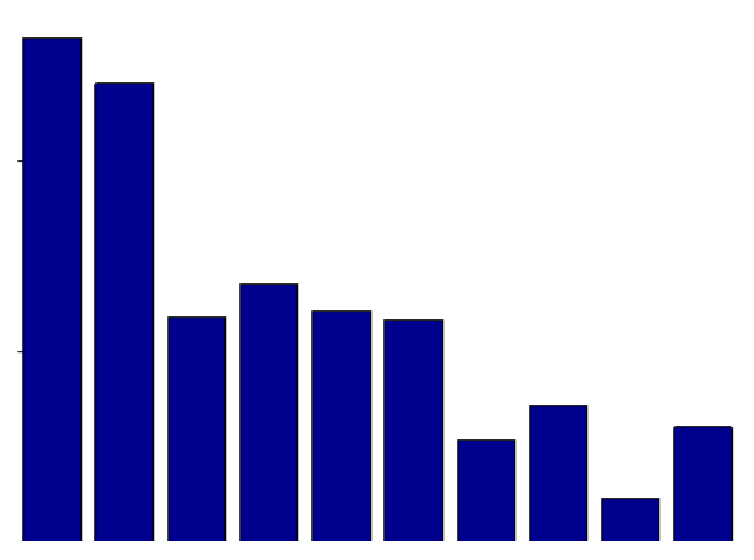
\includegraphics[width=0.24\textwidth, height=8mm]{b2} &
\includegraphics[width=0.24\textwidth, height=8mm]{bb3} &
\includegraphics[width=0.24\textwidth, height=8mm]{bb4} &
\includegraphics[width=0.24\textwidth, height=8mm]{bb5}  \\
\vspace{-10mm}\hspace{0mm}\scalebox{0.72}{
\rotatebox[origin=r]{90}{reaching}\hspace{0.9mm}
\rotatebox[origin=r]{90}{moving}\hspace{0.9mm}
\rotatebox[origin=r]{90}{pouring}\hspace{0.9mm}
\rotatebox[origin=r]{90}{eating}\hspace{0.9mm}
\rotatebox[origin=r]{90}{drinking}\hspace{0.9mm}
\rotatebox[origin=r]{90}{opening}\hspace{0.9mm}
\rotatebox[origin=r]{90}{placing}\hspace{0.9mm}
\rotatebox[origin=r]{90}{closing}\hspace{0.9mm}
\rotatebox[origin=r]{90}{null}\hspace{0.9mm}
\rotatebox[origin=r]{90}{cleaning}}&
\vspace{-10mm}\hspace{-0.9mm}\scalebox{0.72}{
\rotatebox[origin=r]{90}{reaching}\hspace{0.9mm}
\rotatebox[origin=r]{90}{moving}\hspace{0.9mm}
\rotatebox[origin=r]{90}{pouring}\hspace{0.9mm}
\rotatebox[origin=r]{90}{eating}\hspace{0.9mm}
\rotatebox[origin=r]{90}{drinking}\hspace{0.9mm}
\rotatebox[origin=r]{90}{opening}\hspace{0.9mm}
\rotatebox[origin=r]{90}{placing}\hspace{0.9mm}
\rotatebox[origin=r]{90}{closing}\hspace{0.9mm}
\rotatebox[origin=r]{90}{null}\hspace{0.9mm}
\rotatebox[origin=r]{90}{cleaning}}&
\vspace{-10mm}\hspace{-0.9mm}\scalebox{0.72}{
\rotatebox[origin=r]{90}{reaching}\hspace{0.9mm}
\rotatebox[origin=r]{90}{moving}\hspace{0.9mm}
\rotatebox[origin=r]{90}{pouring}\hspace{0.9mm}
\rotatebox[origin=r]{90}{eating}\hspace{0.9mm}
\rotatebox[origin=r]{90}{drinking}\hspace{0.9mm}
\rotatebox[origin=r]{90}{opening}\hspace{0.9mm}
\rotatebox[origin=r]{90}{placing}\hspace{0.9mm}
\rotatebox[origin=r]{90}{closing}\hspace{0.9mm}
\rotatebox[origin=r]{90}{null}\hspace{0.9mm}
\rotatebox[origin=r]{90}{cleaning}}&
\vspace{-10mm}\hspace{-0.9mm}\scalebox{0.72}{
\rotatebox[origin=r]{90}{reaching}\hspace{0.9mm}
\rotatebox[origin=r]{90}{moving}\hspace{0.9mm}
\rotatebox[origin=r]{90}{pouring}\hspace{0.9mm}
\rotatebox[origin=r]{90}{eating}\hspace{0.9mm}
\rotatebox[origin=r]{90}{drinking}\hspace{0.9mm}
\rotatebox[origin=r]{90}{opening}\hspace{0.9mm}
\rotatebox[origin=r]{90}{placing}\hspace{0.9mm}
\rotatebox[origin=r]{90}{closing}\hspace{0.9mm}
\rotatebox[origin=r]{90}{null}\hspace{0.9mm}
\rotatebox[origin=r]{90}{cleaning}}
\end{tabular}
\end{tabular}
\normalsize
\caption{\textbf{Anticipated belief over activity.} In the odd numbered rows, we show a middle frame of the temporal segment. In the even numbered rows, we show the anticipated belief. Note that frames are not visible to the algorithm and only included for evaluation.}
\label{abcd}
\end{figure}


As shown in Figure~\ref{abcd}, anticipated belief is highly accurate. In the first row, the subject is moving the apple, and our algorithm anticipates the next activity accurately as eating. For its consecutive segment, our algorithm relies on the periodic activity of moving and eating/drinking. Hence, it anticipates that the activity following moving should be eating or drinking. In the third row, the initial belief is flatter. Hence, consecutive beliefs are flatter and less informative yet accurate. Moreover, in the fifth row, our algorithm accurately anticipates that box need to be placed after being moved.

%\clearpage
{\small
\bibliography{shortstrings,anticipation_divmrf}
\bibliographystyle{plainnat}

}

\end{document}
